\documentclass[floatsintext,man]{apa6}

\usepackage{amssymb,amsmath}
\usepackage{ifxetex,ifluatex}
\usepackage{fixltx2e} % provides \textsubscript
\ifnum 0\ifxetex 1\fi\ifluatex 1\fi=0 % if pdftex
  \usepackage[T1]{fontenc}
  \usepackage[utf8]{inputenc}
\else % if luatex or xelatex
  \ifxetex
    \usepackage{mathspec}
    \usepackage{xltxtra,xunicode}
  \else
    \usepackage{fontspec}
  \fi
  \defaultfontfeatures{Mapping=tex-text,Scale=MatchLowercase}
  \newcommand{\euro}{€}
\fi
% use upquote if available, for straight quotes in verbatim environments
\IfFileExists{upquote.sty}{\usepackage{upquote}}{}
% use microtype if available
\IfFileExists{microtype.sty}{\usepackage{microtype}}{}

% Table formatting
\usepackage{longtable, booktabs}
\usepackage{lscape}
% \usepackage[counterclockwise]{rotating}   % Landscape page setup for large tables
\usepackage{multirow}		% Table styling
\usepackage{tabularx}		% Control Column width
\usepackage[flushleft]{threeparttable}	% Allows for three part tables with a specified notes section
\usepackage{threeparttablex}            % Lets threeparttable work with longtable

% Create new environments so endfloat can handle them
% \newenvironment{ltable}
%   {\begin{landscape}\begin{center}\begin{threeparttable}}
%   {\end{threeparttable}\end{center}\end{landscape}}

\newenvironment{lltable}
  {\begin{landscape}\begin{center}\begin{ThreePartTable}}
  {\end{ThreePartTable}\end{center}\end{landscape}}




% The following enables adjusting longtable caption width to table width
% Solution found at http://golatex.de/longtable-mit-caption-so-breit-wie-die-tabelle-t15767.html
\makeatletter
\newcommand\LastLTentrywidth{1em}
\newlength\longtablewidth
\setlength{\longtablewidth}{1in}
\newcommand\getlongtablewidth{%
 \begingroup
  \ifcsname LT@\roman{LT@tables}\endcsname
  \global\longtablewidth=0pt
  \renewcommand\LT@entry[2]{\global\advance\longtablewidth by ##2\relax\gdef\LastLTentrywidth{##2}}%
  \@nameuse{LT@\roman{LT@tables}}%
  \fi
\endgroup}


  \usepackage{graphicx}
  \makeatletter
  \def\maxwidth{\ifdim\Gin@nat@width>\linewidth\linewidth\else\Gin@nat@width\fi}
  \def\maxheight{\ifdim\Gin@nat@height>\textheight\textheight\else\Gin@nat@height\fi}
  \makeatother
  % Scale images if necessary, so that they will not overflow the page
  % margins by default, and it is still possible to overwrite the defaults
  % using explicit options in \includegraphics[width, height, ...]{}
  \setkeys{Gin}{width=\maxwidth,height=\maxheight,keepaspectratio}
\ifxetex
  \usepackage[setpagesize=false, % page size defined by xetex
              unicode=false, % unicode breaks when used with xetex
              xetex]{hyperref}
\else
  \usepackage[unicode=true]{hyperref}
\fi
\hypersetup{breaklinks=true,
            pdfauthor={},
            pdftitle={Early language experience in a Tseltal Mayan village},
            colorlinks=true,
            citecolor=blue,
            urlcolor=blue,
            linkcolor=black,
            pdfborder={0 0 0}}
\urlstyle{same}  % don't use monospace font for urls

\setlength{\parindent}{0pt}
%\setlength{\parskip}{0pt plus 0pt minus 0pt}

\setlength{\emergencystretch}{3em}  % prevent overfull lines


% Manuscript styling
\captionsetup{font=singlespacing,justification=justified}
\usepackage{csquotes}
\usepackage{upgreek}

 % Line numbering
  \usepackage{lineno}
  \linenumbers


\usepackage{tikz} % Variable definition to generate author note

% fix for \tightlist problem in pandoc 1.14
\providecommand{\tightlist}{%
  \setlength{\itemsep}{0pt}\setlength{\parskip}{0pt}}

% Essential manuscript parts
  \title{Early language experience in a Tseltal Mayan village}

  \shorttitle{Early language experience in a Tseltal Mayan village}


  \author{Marisa Casillas\textsuperscript{1}, Penelope Brown\textsuperscript{1}, \& Stephen C. Levinson\textsuperscript{1}}

  % \def\affdep{{"", "", ""}}%
  % \def\affcity{{"", "", ""}}%

  \affiliation{
    \vspace{0.5cm}
          \textsuperscript{1} Max Planck Institute for Psycholinguistics  }

  \authornote{
    Correspondence concerning this article should be addressed to Marisa
    Casillas, P.O. Box 310, 6500 AH Nijmegen, The Netherlands. E-mail:
    \href{mailto:Marisa.Casillas@mpi.nl}{\nolinkurl{Marisa.Casillas@mpi.nl}}
  }


  \abstract{Daylong at-home audio recordings from 10 Tseltal Mayan children (ages
0;2--3;0; Southern Mexico) were analyzed for how often children engaged
in verbal interaction with others and whether their speech environment
changed with age, time of day, household size, and number of speakers
present. Children were infrequently directly spoken to, with most
directed speech coming from adults, and no increase with age. Most
directed speech came in the mornings, and interactional peaks contained
nearly four times the baseline rate of directed speech. Coarse
indicators of children's language development (babbling, first words,
first word combinations) suggest that Tseltal children manage to extract
the linguistic information they need despite minimal directed speech.
Multiple proposals for how they might do so are discussed.}
  \keywords{Child-directed speech, linguistic input, non-WEIRD, vocal maturity, turn
taking, interaction, Mayan \\

    \indent Word count: 10561 (8903 not including references)
  }





\usepackage{amsthm}
\newtheorem{theorem}{Theorem}[section]
\newtheorem{lemma}{Lemma}[section]
\theoremstyle{definition}
\newtheorem{definition}{Definition}[section]
\newtheorem{corollary}{Corollary}[section]
\newtheorem{proposition}{Proposition}[section]
\theoremstyle{definition}
\newtheorem{example}{Example}[section]
\theoremstyle{definition}
\newtheorem{exercise}{Exercise}[section]
\theoremstyle{remark}
\newtheorem*{remark}{Remark}
\newtheorem*{solution}{Solution}
\begin{document}

\maketitle

\setcounter{secnumdepth}{0}



\section{Introduction}\label{intro}

A great deal of work in developmental language science revolves around
one central question: what kind of linguistic experience (and how much)
is needed to support first language acquisition? In pursuing this topic,
many researchers have fixed their sights on the speech addressed to
children. In several languages, child-directed speech (CDS, speech
designed for and directed toward a child recipient) has been
demonstrated to be distinct from adult-directed speech (ADS) in that it
is linguistically adapted for young listeners (e.g., Soderstrom, 2007),
interactionally rich (Bruner, 1983), preferred by infants (ManyBabies
Collaborative, 2017), and facilitates early word learning (Cartmill et
al., 2013; Hoff, 2003; Rowe, 2008; Weisleder \& Fernald, 2013).

However, the role of CDS in typical language development is less clear
once we take a broad view of the world's language learning environments.
In any given linguistic community, the vast majority of children acquire
the linguistic system and language behaviors needed for successful
communication in the context in which they are raised. In many cases,
prior ethnographic work suggests that successful adult-like
communicative competence is typically achieved without frequent CDS
(Brown, 2011; de León, 2011; Gaskins, 2006; Ochs \& Schieffelin, 1984).
If so, two important considerations arise: (1) while CDS is a powerful
driver of learning in some contexts, it is unlikely to be universally
fundamental for typical language development (Brown, 2014; Brown \&
Gaskins, 2014), and (2) we should do more to explore other types of
linguistic experience and other features of the learning environment
that allow children to extract the information they need to learn
language.

Past work on child language development in communities with reportedly
infrequent CDS (e.g., Brown, 2011; de León, 2011; Gaskins, 2006; Ochs \&
Schieffelin, 1984) has tended to use rich linguistic and ethnographic
methods that, while well-suited to characterizing language
socialization, lack the quantitative rigor that would otherwise enable
reproducible results derived from reasonably representative participant
samples (but see Shneidman \& Goldin-Meadow, 2012). This situation calls
for work that applies quantitative methods from developmental language
science in diverse ethnolinguistic contexts in order to build more
robust theories of language learning. In this paper we investigate the
language environment and early vocal development of 10 Tseltal Mayan
children growing up in a community where caregivers have been previously
reported to infrequently directly speak to young children (Brown, 1998,
2011, 2014). Our aims are to quantitatively ground these prior
qualitative claims in order to reason about the fundamental factors for
learning language in Tseltal Mayan (and similar) communities.

\subsection{Child-directed speech}\label{intro-cds}

Prior work, conducted primarily in Western contexts, has shown that the
amount of CDS children hear influences their language development; more
CDS is associated with faster-growing receptive and productive
vocabularies (e.g., Hart \& Risley, 1995; Hoff, 2003; Shneidman \&
Goldin-Meadow, 2012), faster lexical retrieval (Weisleder \& Fernald,
2013), and faster syntactic development (Huttenlocher, Waterfall,
Vasilyeva, Vevea, \& Hedges, 2010). Given that CDS is designed for a
child hearer, it is more likely than ADS or other-directed speech to
align with the child's attention, and may thereby facilitate early
language development. There are, however, a few caveats to the body of
work relating CDS quantity and language development. We touch upon three
issues here: its link to grammatical development, its varied use across
activities, and its limited presence in other cultures.

First, while there is overwhelming evidence linking CDS quantity to
vocabulary size, links to grammatical development are more scant (but
see Brinchmann, Braeken, \& Lyster, 2019; Frank, Braginsky, Marchman, \&
Yurovsky, in preparation; Huttenlocher et al., 2010). While the
advantage of CDS for referential word learning is clear, it is less
obvious how it facilitates syntactic learning (Yurovsky, 2018). On the
other hand, there is a wealth of evidence that syntactic knowledge is
lexically specified (e.g., Lieven, Pine, \& Baldwin, 1997), and that,
crosslinguistically, children's vocabulary size is one of the most
robust predictors of their early syntactic development (Frank et al., in
preparation; Marchman, Martínez-Sussmann, \& Dale, 2004)---what is good
for the lexicon may also be good for syntax.

Second, most work on CDS quantity (i.e., how often children hear CDS)
uses summary measures that average over the ebb and flow of the recorded
session. In reality, verbal behaviors are highly temporally structured:
infants' and adults' vocal behavior is clustered across multiple time
scales of daylong recordings (Abney, Smith, \& Yu, 2017), and nouns and
verbs are used within short bursts separated by long periods across
languages (Blasi, Schikowski, Moran, Pfeiler, \& Stoll, in preparation).
In fact, experimental work has shown that children sometimes learn
better from bursty exposure to words (Schwab \& Lew-Williams, 2016).

What's more, the ebbs and flows in children's language exposure are
likely to be associated with different activities during the day, each
of which may carry their own linguistic profile (e.g., vocabulary used
during bookreading vs.~mealtime; Bruner (1983); Tamis-LeMonda, Custode,
Kuchirko, Escobar, and Lo (2018)). Different activities also elicit
different quantities of talk; one study done in Canadian children's
homes and daycares found that the highest density of adult speech came
during storytime and organized playtimes (e.g., sing-alongs,
painting)---activities that contained nearly twice as much talk as
others (e.g., mealtime; Soderstrom \& Wittebolle, 2013). Some of these
activity-driven effects on CDS can even be observed based simply on time
of day given the systematic timing of different activities in children's
daily routines (Greenwood, Thiemann-Bourque, Walker, Buzhardt, \&
Gilkerson, 2011; Soderstrom \& Wittebolle, 2013). If children indeed
benefit from bursty, activity-driven patterns in CDS (Schwab \&
Lew-Williams, 2016)---which appears to be characteristic of their input
(Abney et al., 2017; Blasi et al., in preparation; Bruner, 1983;
Tamis-LeMonda et al., 2018)---researchers should attend more to the
typical range, distribution, and characteristics of the speech they
encounter over the different parts of the day (Greenwood et al., 2011;
Soderstrom \& Wittebolle, 2013).

Third, prior work has typically focused on Western (primarily North
American) populations, limiting our ability to generalize effects of CDS
to children elsewhere (Brown \& Gaskins, 2014; Henrich, Heine, \&
Norenzayan, 2010; M. Nielsen, Haun, Kärtner, \& Legare, 2017). While we
gain valuable insight by looking at within-population variation, we can
more effectively find places where our assumptions break down by
studying language development in communities that diverge meaningfully
(linguistically and culturally) from those already well-studied.
Linguistic anthropologists working in non-Western communities have long
reported that caregiver-child interaction varies immensely from place to
place, place, but that, despite this variation, children do not appear
to show delays in the onset of major communicative benchmarks (e.g.,
pointing, first words; Brown, 2011, 2014; Brown \& Gaskins, 2014;
Gaskins, 2006; Liszkowski, Brown, Callaghan, Takada, \& de Vos, 2012;
Ochs \& Schieffelin, 1984). These findings have had a limited impact on
mainstream theories of language development, partly due to a lack of
directly comparable methods (Brown, 2014; Brown \& Gaskins, 2014).

A number of recent or ongoing research projects have used standard
psycholinguistic methods to investigate language learning environments
in traditional, non-Western communities, with several substantiating the
claim that children in many parts of the world hear little CDS. Scaff,
Cristia, and colleagues (2017; in preparation) estimate, based on
daylong recordings, that Tsimane children (Bolivian lowlands;
forager-horticulturalist) hear approximately 4.8 minutes of CDS per hour
between ages 0;6 and 3;0 when considering all possible environmental
speech (Cristia et al., 2017; Scaff et al., in preparation; see also
work by Vogt, Mastin, and Schots (2015) with Mozambican infants).
Shneidman and Goldin-Meadow (2012) analyzed speech from one-hour at-home
video recordings of children between 1;0 and 3;0 in a Yucatec Mayan and
a North American community. Their analyses yielded four main findings:
compared to the American children, (a) Yucatec children heard many fewer
utterances per hour, (b) a much smaller proportion of the utterances
they heard were child-directed, (c) the proportion of utterances that
were child-directed increased dramatically with age, matching U.S.
children's CDS proportion by 3;0, and (d) most of the added CDS in the
Yucatec sample came from other children (e.g., older siblings/cousins).
The lexical diversity of the CDS that Yucatec Mayan children heard at 24
months---particularly from adult speakers---predicted their vocabulary
knowledge at 35 months, suggesting that CDS characteristics still play a
role in that context. Notably, links between activity-type and CDS
(e.g., Soderstrom \& Wittebolle, 2013) have not yet been systematically
investigated in any non-WEIRD community; known high-density CDS
activities (e.g., bookreading) are reported to be vanishingly rare in
some of these communities, and so the peaks in interactive talk may be
associated with different routine activities at different times of day.

The current study aimed to address two of these three issues by using
both daylong audio recordings and standard measures of vocal development
to better understand how much CDS Tseltal Mayan children hear over the
first three years of life, what times of day they are most likely to
hear CDS, and how their spontaneous vocalizations change in maturity
during that same period.

\subsection{Vocal maturity of spontaneous
speech}\label{vocal-maturity-of-spontaneous-speech}

Past ethnographic work has reported that, despite hearing little CDS,
children in some contexts show no evidence of language delay (e.g.,
Brown, 2011, 2014; Brown \& Gaskins, 2014; Liszkowski et al., 2012). We
test this claim by comparing Tseltal children's achievement of major
speech production milestones to those already known for Western
children. In so doing, we report on the \enquote{vocal maturity} of
Tseltal children's spontaneous speech (i.e., use of adult-like
production types). Our vocal maturity measure is designed to capture the
transition from (a) non-canonical babble to canonical
(\enquote{speech-like}) babble, (b) canonical babble to first words, and
(c) single-word utterances to multi-word utterances. This measure is, at
best, a coarse approximation of children's true linguistic abilities,
but it is an efficient means for getting a bird's eye view of children's
speech as it becomes more linguistically complex over the first three
years.

Importantly, children's vocal maturity may be more subject to
environmental factors as they grow older. The onset of canonical
babbling during the first year appears to be overall relatively stable
in response to variable language environments (e.g., Lee, Jhang, Relyea,
Chen, \& Oller, 2018; Oller, Eilers, Basinger, Steffens, \& Urbano,
1995; Oller, Eilers, Neal, \& Cobo-Lewis, 1998). That said, there is
variation in the precise onset age of canonical babble; one longitudinal
study showed an onset age range of 0;9 to 1;3 among children from a
relatively homogenous middle-class sample (McGillion et al., 2017). The
same study showed that the age of onset for canonical babbling
significantly predicted the age of onset for first words. Once children
begin producing recognizable words, environmental effects become more
apparent; vocabulary size---even very early vocabulary---is known to be
sensitive to language environment factors such as maternal education and
birth order (see, e.g., Frank et al., in preparation). Early vocabulary
size is also a robust cross-linguistic predictor of later syntactic
development, including the age at which a child is likely to have begun
combining words (Frank et al., in preparation; Marchman et al., 2004).

Therefore, if we indeed find that Tseltal children hear relatively
little CDS, one might expect that the emergence of canonical babble
would occur around the same age as it does in Western children, but that
the emergence of single words and multi-word utterances would diverge
from known middle-class Western norms.

\subsection{The current study}\label{intro-currentstudy}

We examined the early language experience of 10 Tseltal Mayan children
under age 3;0 using daylong photo-linked audio recordings. Prior
ethnographic work suggests that Tseltal caregivers do not frequently
directly speak to their children until the children themselves begin to
actively initiate verbal interactions (Brown, 2011, 2014). Nonetheless,
Tseltal children develop language with no apparent delays (Brown, 2011,
2014; Liszkowski et al., 2012; see also Pye, 2017). We provide more
details on the community and dataset in the
\protect\hyperlink{methods}{Methods section}. We analyzed two basic
measures of Tseltal children's language environments: (a) the quantity
of speech directed to them (TCDS; target-child-directed speech) and (b)
the quantity of other-directed speech (ODS; speech directed to anyone
but the target child). We also then coarsely outline children's
linguistic development using vocal maturity estimates from their
spontaneous vocalizations.

Based on prior work, we predicted that Tseltal Mayan children would be
infrequently directly addressed, that the amount of TCDS would increase
with age, that most TCDS would come from other children, that TCDS would
be most common during the morning and afternoon family gatherings, and
that children's early vocal development would show no sign of delay with
respect to known Western onset benchmarks.

\hypertarget{methods}{\section{Method}\label{methods}}

\subsection{Corpus}\label{methods-dataset}

The children in this dataset come from a small-scale, subsistence
farming community in the highlands of Chiapas (Southern Mexico). The
vast majority of children in the community grow up speaking Tseltal
monolingually at home. Nuclear families are typically organized into
patrlineal clusters of large, multi-generation households. Tseltal
children's language environments have previously been characterized as
non-child-centered and non-object-centered (Brown, 1998, 2011, 2014).

During their waking hours, young infants are typically tied to their
mother's back while she goes about her daily activities. The arc of a
typical day for a mother might include waking and dressing for the day,
a meal including most of the household, dispersal of household members
for work in the field, at home, or elsewhere, a late afternoon snack
with the most of the household now back home, visiting nearby family,
food preparation for the next day, a final meal, and then dispersal for
evening activities and, when it comes, sleep. If the mother goes to work
in the field, the infant is sometimes left with other family members at
home (e.g., an aunt or sibling), but is sometimes taken along. Young
children are often cared for by other family members, especially older
siblings, and may themselves begin to help watch their infant siblings
once they reach age three and older.

Typically, TCDS is limited until children themselves begin to initiate
interactions, usually around age 1;0. Interactional exchanges, when they
do occur, are often brief or non-verbal (e.g., object exchange routines)
and take place within a multi-participant context (Brown, 2014).
Interactions tend to focus on appropriate actions and responses (not on
words and their meanings), and young children are socialized to attend
to the activities taking place around them (see also de León, 2011;
Rogoff, Paradise, Arauz, Correa-Chávez, \& Angelillo, 2003). By age
five, most children are competent speakers who engage in daily chores
and the caregiving of their younger siblings. The Tseltal approach to
caregiving is similar to that described for other Mayan communities
(e.g., de León, 2011; Gaskins, 2000; Pye, 1986; Rogoff et al., 2003;
Shneidman \& Goldin-Meadow, 2012).

The current data come from (corpus name and references retracted for
review), which includes raw daylong recordings and other developmental
language data from more than 100 children under 4;0 across two
traditional indigenous communities: the Tseltal Mayan community
described here and a Papua New Guinean community described elsewhere
(reference retracted for review). This Tseltal corpus, primarily
collected in 2015, includes raw recordings from 55 children born to 43
mothers. The participating families typically only had 2 to 3 children
(median = 2; range = 1--9), due to the fact that they come from a young
subsample of the community (mothers: mean = 26.3 years; median = 25;
range = 16--43 and fathers: mean = 30; median = 27; range = 17---52).
Based on the ages of living children, we estimate that, on average,
mothers were 20 years old when they had their first child (median = 19;
range = 12--27), with a following average inter-child interval of 3
years (median = 2.8; range = 1--8.5). Twenty-eight percent of the
participating families had two children under 4;0. Household size,
defined in our dataset as the number of people sharing a kitchen or
other primary living space, ranged between 3 and 15 people (mean = 7.2;
median = 7). Although 32.7\% of the target children are first-born, they
were rarely the only child in their household. Most mothers had finished
primary school (37\%; 6 years of education) or secondary school (30\%; 9
years of education), with a few more having completed preparatory school
(12\%; 12 years of education) or some university-level training (2\%
(one mother); 16 years of education); the remainder (23\%) had no
schooling or did not complete primary school. All fathers had finished
primary school, with most completing secondary school (44\%) or
preparatory school (21\%), and two completing some university-level
training (5\%). To our knowledge at the time of recording, all children
were typically developing.

When possible, we collected dates of birth for children using a medical
record card typically provided by the local health clinic within two
weeks of birth. However, some children do not have this card and
sometimes cards are created long after a child's birth. We asked all
parents to also tell us the approximate date of birth of the child, the
child's age, and an estimate of the time between the child's birth and
creation of the medical record card. We used these multiple sources of
information to triangulate the child's most likely date of birth if the
medical record card appeared to be unreliable, following up for more
details from the families if necessary.

We used a novel combination of a lightweight stereo audio recorder
(Olympus WS-832) and wearable photo camera (Narrative Clip 1) fitted
with a fish-eye lens to track children's interactions over the course of
a 9--11-hour period at home in which the experimenter was not present.
Ambulatory children wore both devices at once (as shown in
\protect\hyperlink{fig1}{Figure 1}) while other children wore the
recorder in a onesie while their primary caregiver wore the camera on an
elastic vest. The camera was set to take photos at 30-second intervals
and was synchronized to the audio in post-processing to generate
snapshot-linked audio (media post-processing scripts at:
\url{https://github.com/retracted_for_review}). We used these recordings
to capture a wide range of the linguistic patterns children encounter as
they participate in different activities over the course of their day
(Bergelson, Amatuni, Dailey, Koorathota, \& Tor, 2018; Greenwood et al.,
2011; Tamis-LeMonda et al., 2018).

\begin{figure}

{\centering 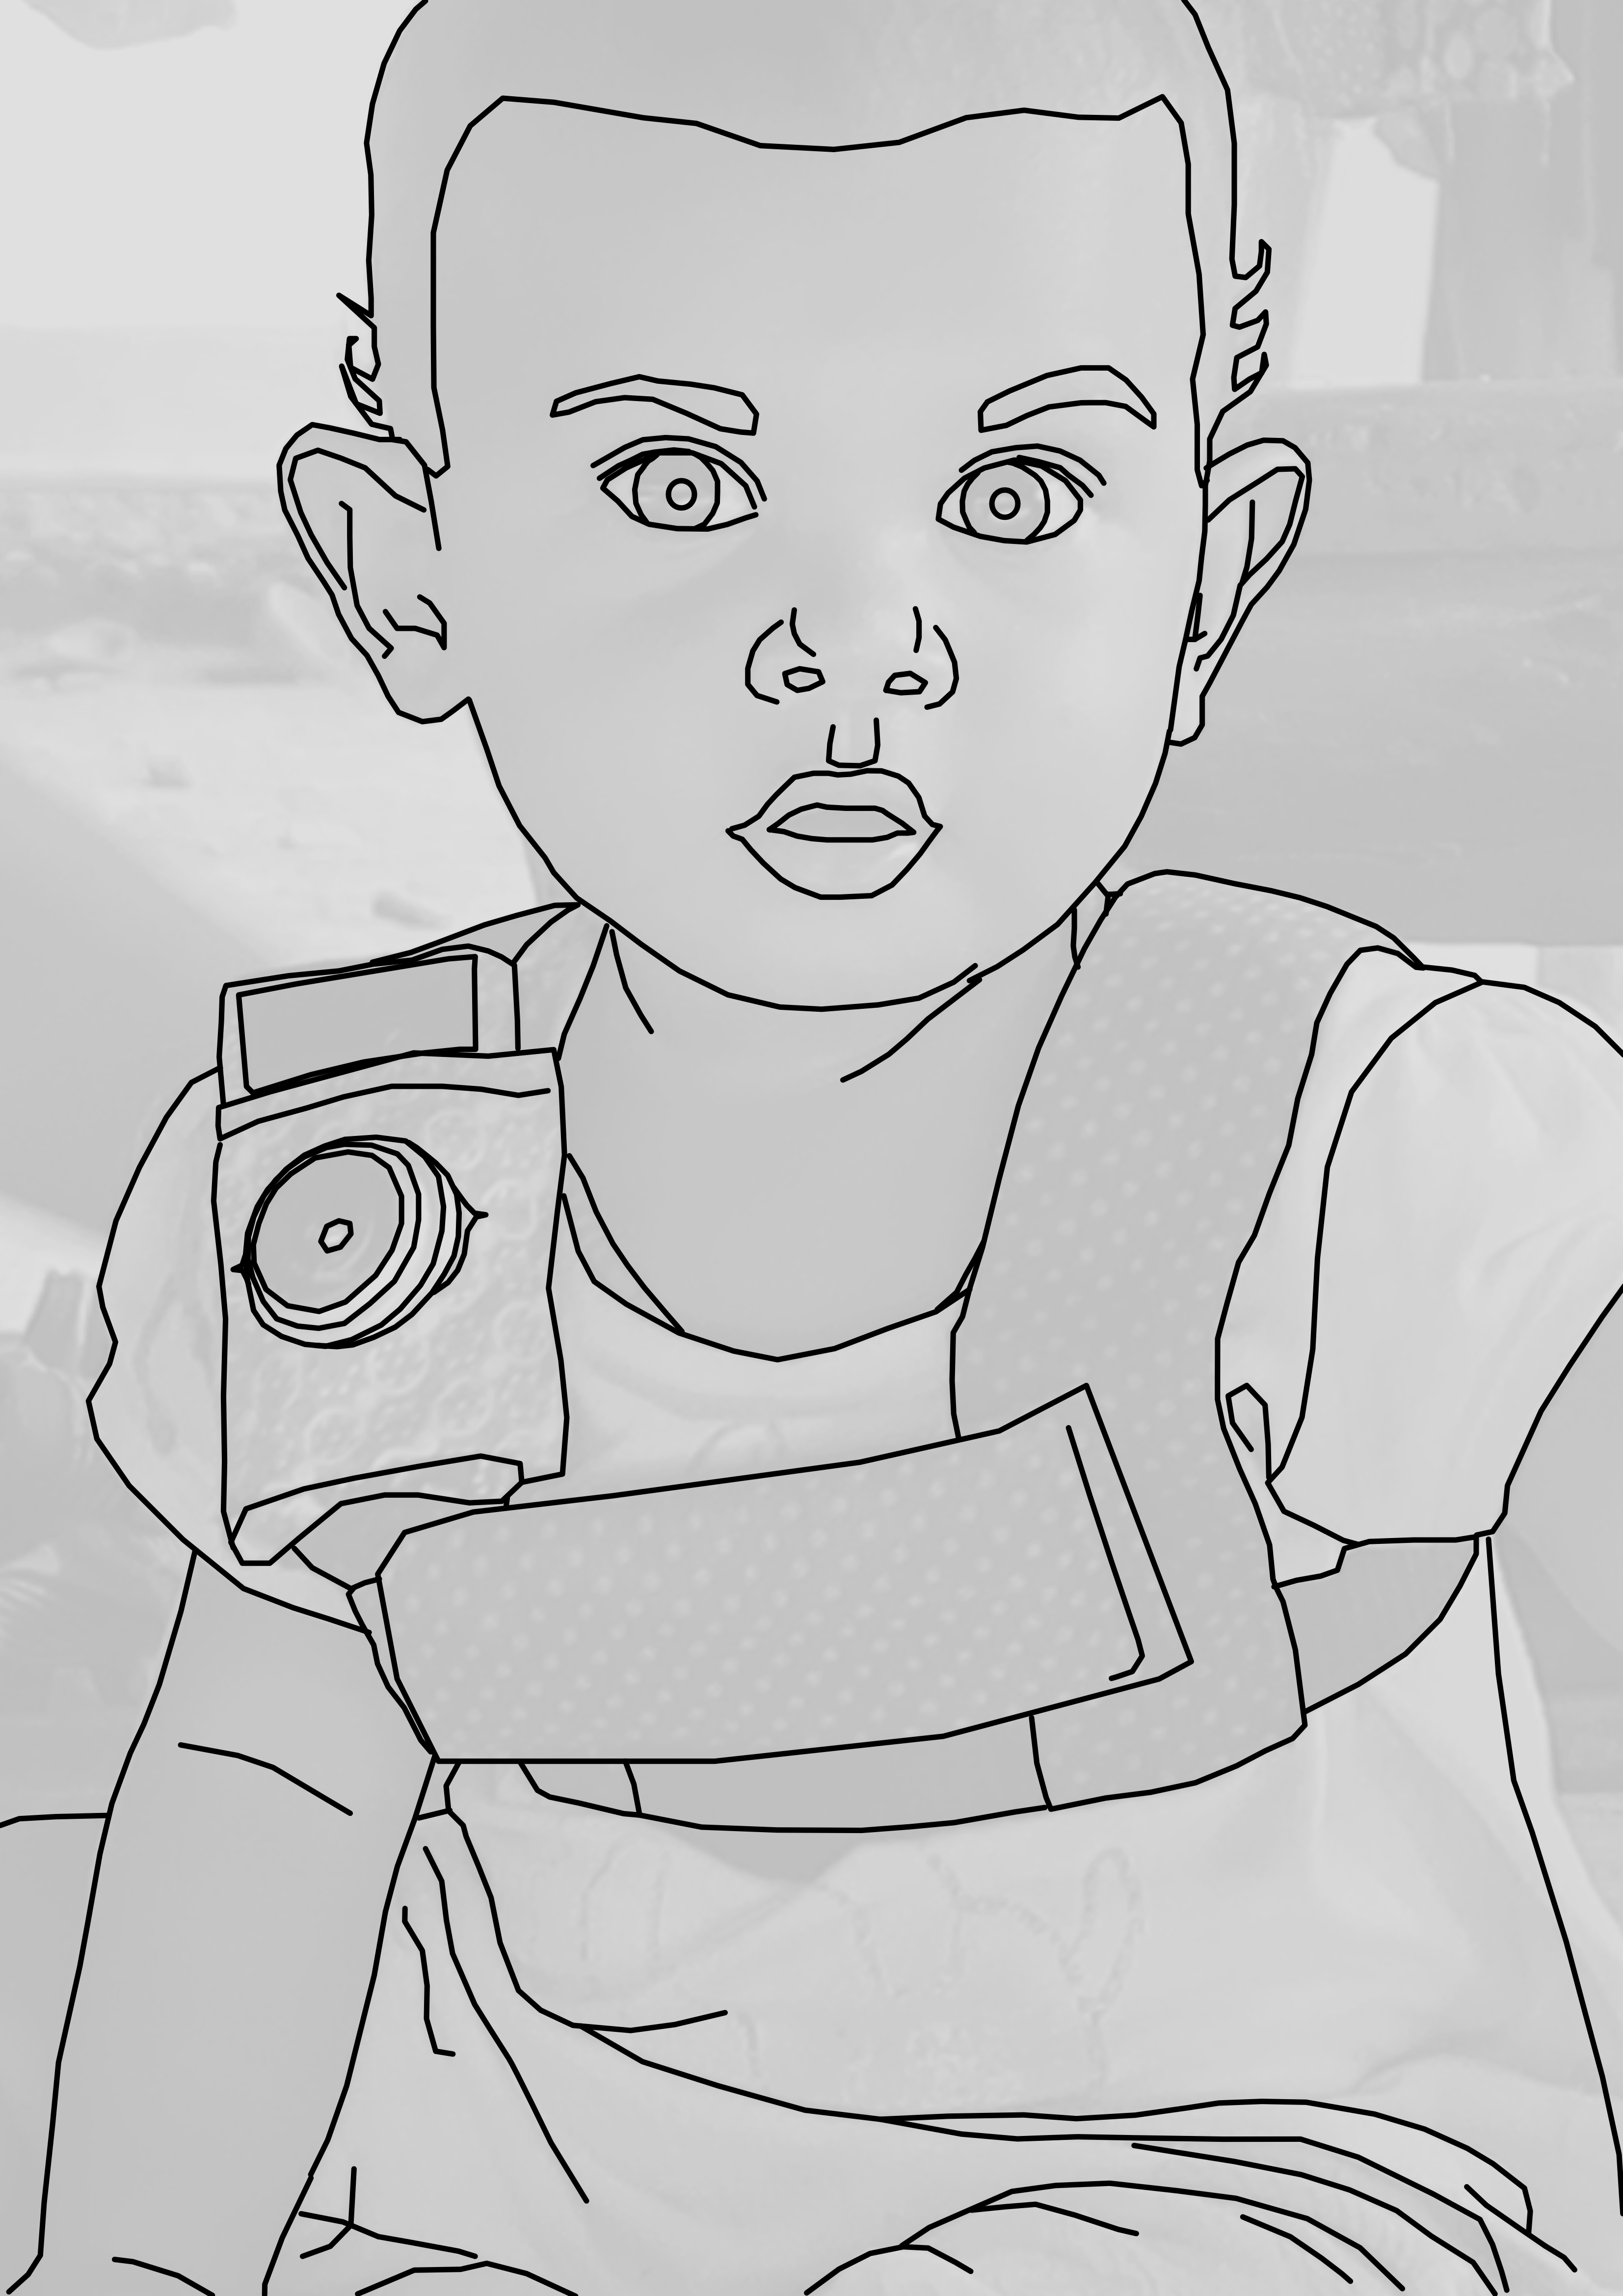
\includegraphics[width=0.3\linewidth]{Tseltal-CLE_files/TseltalCLE-RecordingVest} 

}

\caption{The recording vest included an Olympus audio recorder in the front horizontal pocket and a miniature camera with a fish-eye lens on the shoulder strap.}\label{fig:fig1}
\end{figure}

\subsection{Data selection and annotation}\label{methods-samples}

Although the Tseltal corpus contains more than 500 hours of raw
photo-linked audio, very little of it is useful without adding manual
annotation. We estimated that we could fully transcribe approximately 10
hours of the corpus over the course of three 6-week field stays in the
village between 2015 and 2018, given full-time help from a native member
of the community on each trip. This estimate was approximately correct:
average exhaustive transcription time for one minute of audio was around
50 minutes, given that many clips featured overlapping multi-speaker
talk and/or significant background noise. Given the resource-intensive
nature of annotation, we strategically sampled clips in a way that would
let us ask about age-related changes in children's language experience,
but with enough data per child to generate accurate estimates of their
individual speech environments (see also retracted for review). Our
solution was as follows:

We chose 10 children's recordings based on maximal spread in child age
(0;0--3;0), child sex, and maternal education
(\protect\hyperlink{tab1}{Table 1}; all had native Tseltal-speaking
parents). We selected one hour's worth of non-overlapping clips for
transcription from each recording in the following order: nine randomly
selected 5-minute clips, five manually selected 1-minute top
\enquote{turn-taking} clips, five manually selected 1-minute top
\enquote{vocal activity} clips, and one manually selected 5-minute
extension of the best 1-minute clip (see \protect\hyperlink{fig2}{Figure
2} for an overview of sample distribution within the recordings). The
idea in creating these different subsamples was to measure properties of
(a) children's \emph{average} language environments, (b) their most
\emph{input-dense} language environments, and (c) their most
\emph{mature vocal behavior}, known as the \enquote{random},
\enquote{turn-taking}, and \enquote{vocal activity} samples,
respectively. All the samples were taken between the moment experimenter
departed and the moment she returned.

\begin{table}[tbp]
\begin{center}
\begin{threeparttable}
\caption{\label{tab:tab1}Demographic overview of the 10 children whose recordings are sampled in the current study, including from left to right: child's age (Years;Months.Days); child's sex (M/F); mother's age (years); level of maternal education (none/primary/secondary/preparatory/university); and the number of people living in the child's household.}
\begin{tabular}{lllll}
\toprule
Age & \multicolumn{1}{c}{Sex} & \multicolumn{1}{c}{Mother's age} & \multicolumn{1}{c}{Level of maternal education} & \multicolumn{1}{c}{People in household}\\
\midrule
0;01.25 & M & 26 & none & 8\\
0;03.18 & M & 22 & preparatory & 9\\
0;05.29 & F & 17 & secondary & 15\\
0;07.15 & F & 24 & primary & 9\\
0;10.21 & M & 24 & secondary & 5\\
1;02.10 & M & 21 & none & 9\\
1;10.03 & F & 31 & preparatory & 9\\
2;02.25 & F & 17 & primary & 5\\
2;08.05 & F & 28 & secondary & 5\\
3;00.02 & M & 28 & primary & 6\\
\bottomrule
\end{tabular}
\end{threeparttable}
\end{center}
\end{table}

The turn-taking and high-activity clips were chosen by two trained
annotators (the first author and a student assistant) who listened to
each raw recording in its entirety at 1--2x speed while actively taking
notes about potentially useful clips. The first author then reviewed the
list of candidate clips and chose the best five 1-minute samples for
each of the two activity types. Note that, because the manually selected
clips did not overlap with the initial \enquote{random} clip selection,
the \enquote{true} peak turn-taking and vocal-activity clips for the day
could have possibly occurred during the random clips. High-quality
turn-taking activity was defined as closely timed sequences of
contingent vocalization between the target child and at least one other
person (i.e., frequent vocalization exchanges). High-quality vocal
activity clips were defined as periods in which the target child
produced the most and most diverse spontaneous (i.e., not imitative)
vocalizations (full instructions at
\url{https://git.io/retracted_for_review}).

\begin{figure}
\centering
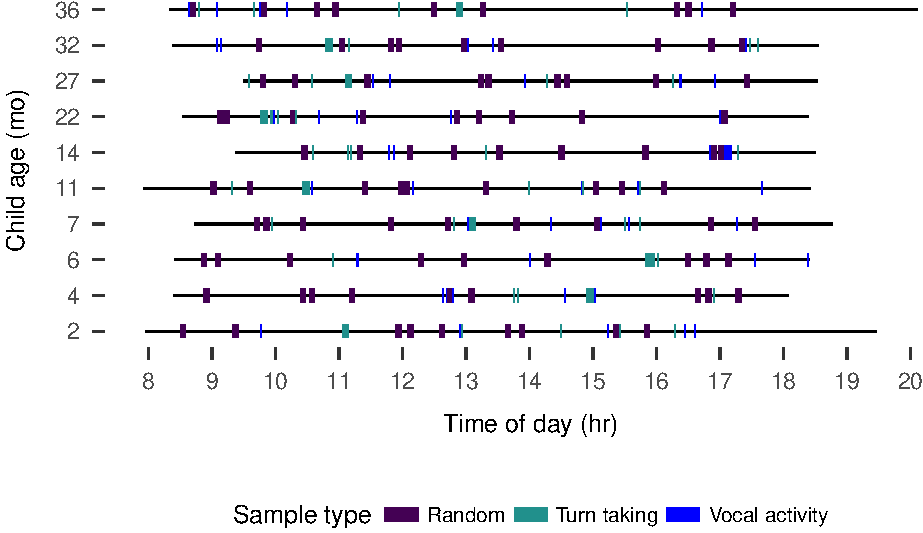
\includegraphics{Tseltal-CLE_files/figure-latex/fig2-1.pdf}
\caption{\label{fig:fig2}Recording duration (black line) and sampled clips
(colored boxes) for each of the 10 recordings analyzed, sorted by child
age in months.}
\end{figure}

The 10 hours of clips were then jointly transcribed and annotated by the
first author and a native speaker of Tseltal who personally knows all
the recorded families. Transcription was done in ELAN (Wittenburg,
Brugman, Russel, Klassmann, \& Sloetjes, 2006) using the ACLEW
Annotation Scheme (full documentation at
\url{https://osf.io/b2jep/wiki/home/}, Casillas et al., 2017).
Utterance-level annotations included: an orthographic transcription
(Tseltal), a loose translation (Spanish), a vocal maturity rating for
each target child utterance (non-linguistic/non-canonical
babbling/canonical babbling/single words/multiple words), and the
intended addressee type for all non-target-child utterances
(target-child/other-child/adult/adult-and-child/animal/other-speaker-type).
Intended addressee was determined using contextual and interactional
information from the photos, audio, and preceding and following footage;
utterances with no clear intended addressee were marked as
\enquote{unsure}. We annotated lexical utterances as single- or
multi-word based on the word boundaries provided by the single native
speaker who reviewed all transcriptions; Tseltal is a mildly
polysynthetic language (words typically contain multiple morphemes).
Note that we did not annotate individual activity types in the clips; we
instead use time of day as a proxy for the activities and daily routines
associated with subsistence farming and family life in this community
(see above).

\subsection{Data analysis}\label{methods-analysisinfo}

In what follows we first describe Tseltal children's speech environments
based on the nine randomly selected 5-minute clips from each child. We
investigate the effects of child age, time of day, household size, and
number of speakers on both TCDS min/hr and ODS min/hr. We then repeat
these analyses, only now looking at the high \enquote{turn-taking}
clips. Finally, we wrap up by outlining a coarse trajectory of Tseltal
children's early vocal development.

\subsection{Statistical models}\label{statistical-models}

All analyses were conducted in R with generalized linear mixed-effects
regressions using the glmmTMB package, and all plots were generated with
ggplot2 (M. E. Brooks et al., 2017; R Core Team, 2018; Wickham, 2009).
All data and analysis code can be found at
\url{https://github.com/retracted_for_review} (temporarily available as
an anonymous OSF repository:
\url{https://osf.io/9xd5u/?view_only=03a351c1172f4d17af9fce634aefb65e})
Notably, both speech environment measures are naturally restricted to
non-negative (0--infinity) values. This implicit boundary restriction at
zero causes the distributional variance of the measures to become
non-gaussian (i.e., with a long right tail). We handle this issue by
using a negative binomial linking function in the regression, which
estimates a dispersion parameter (in addition to the mean and variance)
that allows the model to more closely fit our non-negative,
overdispersed data (M. E. Brooks et al., 2017; Smithson \& Merkle,
2013). When, in addition to this, extra cases of zero were evident in
the distribution (e.g., TCDS min/hr was zero because the child was
alone), we also added a zero-inflation model to the regression. A
zero-inflation negative binomial regression creates two models: (a) a
binary model to evaluate the likelihood of none vs.~some presence of the
variable (e.g., no vs.~some TCDS) and (b) a count model of the variable
(e.g., \enquote{3} vs. \enquote{5} TCDS min/hr), using the negative
binomial distribution as the linking function. Alternative, gaussian
linear mixed-effects regressions with logged dependent variables are
available in the Supplementary Materials, but the results are broadly
similar to what we report here.

\section{Results}\label{results}

Our model predictors were as follows: child age (months), household size
(number of people), and number of non-target-child speakers present in
that clip, all centered and standardized, plus time of day at the start
of the clip (as a factor; \enquote{morning} = up until 11:00;
\enquote{midday} = 11:00--13:00; and \enquote{afternoon} = 13:00
onwards). In addition, the model inluded two-way interactions between
child age and: (a) the number of speakers present, (b) household size,
and (c) time of day. We also added a random effect of child. For the
zero-inflation models, we included the number of speakers present. We
only report significant effects in the main text; full model outputs are
available in the Supplementary Materials.

\begin{figure}
\centering
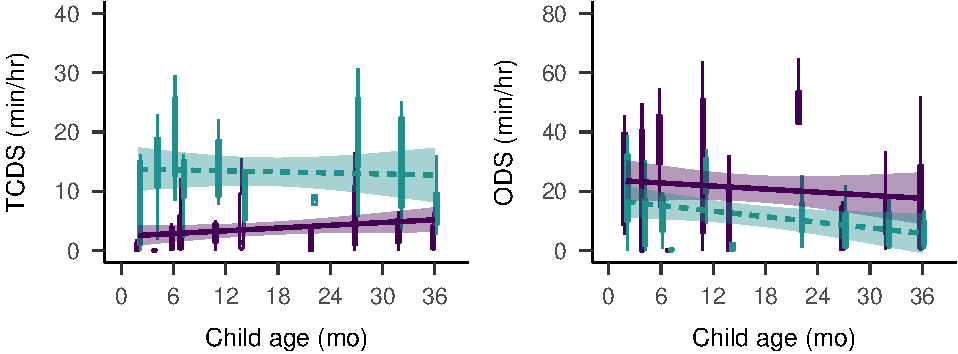
\includegraphics{Tseltal-CLE_files/figure-latex/fig3-1.pdf}
\caption{\label{fig:fig3}Estimates of TCDS min/hr (left) and ODS min/hr
(right) across the sampled age range. Each box plot summarizes the data
for one child from the randomly sampled clips (purple; solid) or the
turn taking clips (green; dashed). Bands on the linear trends show 95\%
confidence intervals.}
\end{figure}

\begin{figure}
\centering
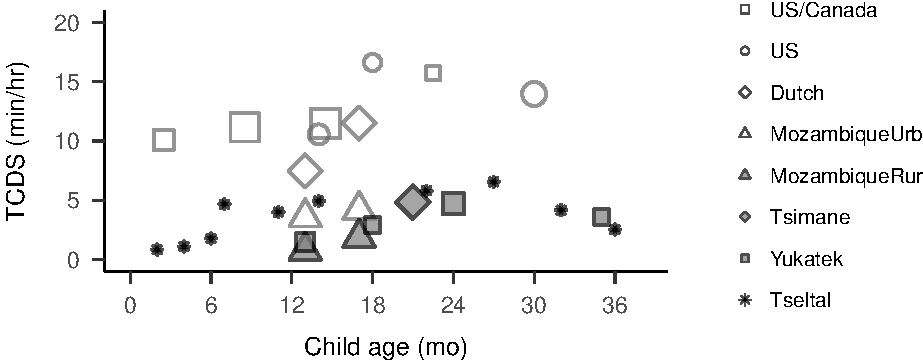
\includegraphics{Tseltal-CLE_files/figure-latex/fig4-1.pdf}
\caption{\label{fig:fig4}Average CDS rates reported from at-home recordings
across various populations and ages, including urban (empty shape) and
rural or indigenous (filled shape) samples. Point size indicates the
number of children represented (range = 1--26). Data sources: Bergelson
et al. (2019) US/Canada; Shneidman (2010) US and Yucatec; Vogt et al.
(2015) Dutch, Mozambique urban and rural; Scaff et al. (in preparation)
Tsimane.}
\end{figure}

\subsection{Target-child-directed speech
(TCDS)}\label{target-child-directed-speech-tcds}

The children in our sample were directly spoken to for an average of
3.63 minutes per hour in the random sample (median = 4.08; range =
0.83--6.55; \protect\hyperlink{fig3}{Figure 3}). These estimates are
similar to those reported for Yucatec Mayan children (Shneidman \&
Goldin-Meadow, 2012), as illustrated in \protect\hyperlink{fig4}{Figure
4} (see Scaff et al. (in preparation) for more detailed cross-language
comparisons). Note that, to make this comparison, we have converted
Shneidman's (2010) utterance/hr estimates to min/hr using the median
Tseltal utterance duration for non-target child speakers (1029 msec),
motivated by the fact that Yucatec and Tseltal are related languages
spoken in comparably rural indigenous communities.

We modeled TCDS min/hr in the random clips with a zero-inflated negative
binomial regression. TCDS rate numerically increased with age, but the
effect was not significant (B = 0.60, SD = 0.36, z = 1.68, p = 0.09).
The rate of TCDS in the randomly sampled clips \emph{was} affected by
factors relating to the time of day (see \protect\hyperlink{fig5}{Figure
5} for an overview of time-of-day findings). The count model showed that
the children were more likely to hear TCDS in the mornings than at
midday (B = 0.83, SD = 0.40, z = 2.09, p = 0.04), with no difference
between morning and afternoon (p = 0.21) or midday and afternoon (p =
0.19). These time-of-day effects also varied by age: while younger
children heard little TCDS from midday onwards, older children showed a
significantly larger decrease in TCDS only in the afternoon; TCDS rates
in the afternoon were significantly lower for older children than they
were at midday (B = -0.85, SD = 0.38, z = -2.26, p = 0.02) and
marginally lower than they were morning (B = 0.57, SD = 0.30, z = 1.90,
p = 0.06). Older target children were also significantly more likely to
hear TCDS when more speakers were present, compared to younger children
(B = 0.57, SD = 0.19, z = 2.95, p \textless{} 0.01). There were no other
significant effects in either the count or the zero-inflation model.

\begin{figure}
\centering
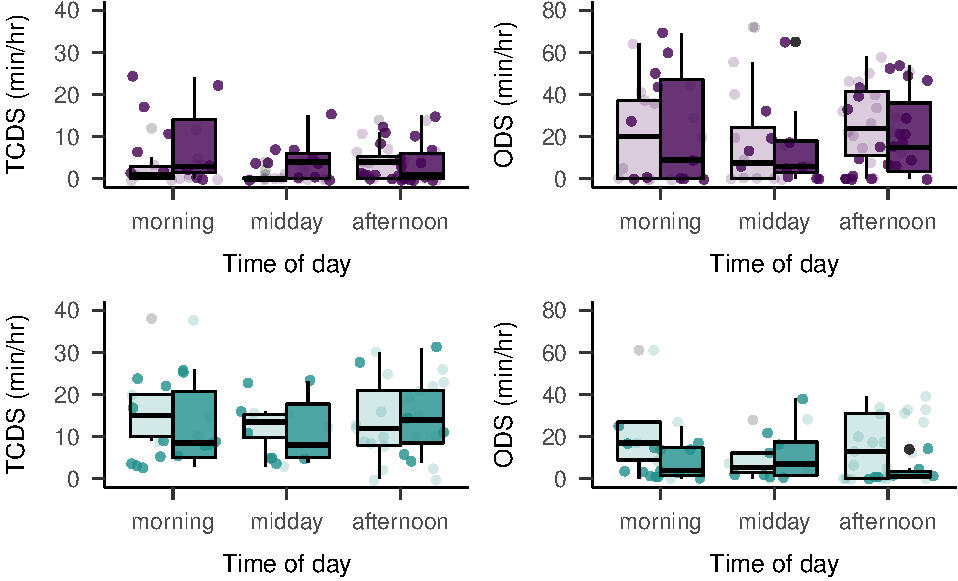
\includegraphics{Tseltal-CLE_files/figure-latex/fig5-1.pdf}
\caption{\label{fig:fig5}Estimates of TCDS min/hr (left panels) and ODS
min/hr (right panels) across the recorded day in the random clips (top
panels) and turn-taking (bottom panels) clips. Each box plot summarizes
the data for children age 1;0 and younger (light) or age 1;0 and older
(dark) at the given time of day.}
\end{figure}

In contrast to findings from Shneidman and Goldin-Meadow (2012) on
Yucatec Mayan, most TCDS in the current data came from adult speakers
(mean = 80.61\%, median = 87.22\%, range = 45.90\%--100\%), with no
evidence that TCDS from \emph{other} children increases with target
child age (Spearman's \emph{rho} = -0.29; \emph{p} = 0.42). Among
adults, the vast majority of TCDS came from women: 4 children heard no
adult male TCDS at all in the samples and, between the other 6 children,
women spoke to children an average of 16.77 times longer than men did
(median = 12.23, range = 0.94--55.64).

\subsection{Other-directed speech
(ODS)}\label{other-directed-speech-ods}

Children heard an average of 21.05 minutes of ODS per hour in the random
sample (median = 17.80; range = 3.57--42.80): that is, nearly six times
as much speech as was directed to them, on average. We modeled ODS
min/hr in the random clips with a zero-inflated negative binomial
regression. The count model of ODS in the randomly selected clips
revealed a significant decrease with child age (B = -0.39, SD = 0.16, z
= -2.43, p = 0.02). In addition to this decrease in age, the model also
revealed that the presence of more speakers was strongly associated with
more ODS (B = 0.68, SD = 0.09, z = 7.29, p \textless{} 0.001). There
were an average of 3.44 speakers present other than the target child in
the randomly selected clips (median = 3; range = 0--10), more than half
of whom were typically adults.

ODS was also strongly affected by time of day
(\protect\hyperlink{fig5}{Figure 5}), showing its lowest point overall
around midday. Compared to midday, target children were overall
significantly more likely to hear ODS in both the mornings (B = 0.45, SD
= 0.18, z = 2.49, p = 0.01) and the afternoons (B = 0.33, SD = 0.16, z =
1.99, p = 0.05), with no significant difference between ODS rates in the
mornings and afternoons (p = 0.41). As before, ODS rate varied across
the day depending on the target child's age: the increase in ODS between
the midday and afternoon was significantly larger for older children (B
= 0.42, SD = 0.17, z = 2.42, p = 0.02), with no significant differences
in child age for the morning-to-midday difference (p = 0.19) or the
difference between morning and afternoon (p = 0.33). There were no other
significant effects on ODS rate, and no significant effects in the
zero-inflation models.

\subsection{TCDS and ODS during interactional
peaks}\label{tcds-and-ods-during-interactional-peaks}

The estimates just given for TCDS and ODS are based on a random sample
of clips from the day; they represent baseline rates of speech in
children's environment and the overall effects of child age, time of
day, and number of speakers on the rates of speech. We could instead
investigate these measures using clips where we know interaction is
taking place: how much speech do children hear during the interactional
peaks that are distributed throughout the day? To answer this question
we repeated the same analyses of TCDS and ODS as above, only this time
using the high turn-taking clips in the sample instead of the random
ones (see the green/dashed summaries in \protect\hyperlink{fig3}{Figures
3} and \protect\hyperlink{fig5}{5}).

Children heard much more TCDS in the turn-taking clips---13.28 min/hr
(nearly 4x the random sample rate; median = 13.65; range =
7.32--20.19)---while also hearing less ODS---11.93 min/hr (nearly half
the random sample rate; median = 10.18; range = 1.37--24.42). We
analyzed both TCDS and ODS rate with parallel models to those used for
the random sample, though this time we did not include a zero-inflation
component for TCDS given that the child was, by definition, directly
addressed at least once in these clips (i.e., there were no cases of
zero TCDS in the turn-taking sample). Full model outputs are available
in the Supplementary Materials.

The models revealed that none of the predictors---child age, time of
day, household size, number of speakers present, or their
combinations---significantly impacted the rate of TCDS children heard
during peak interactivity clips. Put another way, although child age,
time of day, and number of speakers impacted the pattern of TCDS when
viewing children's linguistic input in the \emph{random} baseline, none
of these factors significantly predicted the rate of TCDS used when we
only look at the interactive peaks for the day, probably because the
TCDS rate in this set of clips is near the ceiling of what caregivers do
when interacting with young children.

In the model of ODS, we still saw a significant decrease with child age
(B = -0.80, SD = 0.23, z = -3.43, p = \textless{} 0.001) and a
significant increase when more speakers were present (B = 0.63, SD =
0.10, z = 6.44, p = \textless{} 0.01). This result suggests that child
age and the number of speakers present are robust predictors of ODS
quantity across different language environment contexts.

The rate of ODS during interactional peaks was also still impacted by
time of day, but the lowest point in ODS came later, in the afternoon,
rather than at midday (morning-vs-afternoon: B = -0.61, SD = 0.25, z =
-2.41, p = 0.02; afternoon-vs-midday: B = 0.61, SD = 0.29, z = 2.07, p =
0.04), with no difference between ODS rates at morning and midday (p =
0.99) and no interactions between child age and time of day. Finally,
the model also revealed an unexpected significant decrease in ODS with
increased household size (B = -0.18, SD = 0.09, z = -2.12, p = 0.03), a
result we come back to in the \protect\hyperlink{disc}{Discussion
section}.

In sum, our results provide compelling evidence in support of prior work
claiming that Tseltal children hear very little directly addressed
speech (Brown, 1998, 2011, 2014) and that their speech input is
non-uniformly distributed over the course of the day (Abney et al.,
2017; Blasi et al., in preparation), primarily in the mornings (TCDS and
ODS) and afternoons (ODS), when most of the household is likely to be
present. Do Tseltal children then show any obvious evidence of delay in
their early vocal development?

\subsection{Vocal maturity}\label{vocal-maturity}

We assessed whether the Tseltal children's vocalizations demonstrated
transitions from (a) non-canonical babble to canonical babble, (b)
canonical babble to first words, and (c) single-word utterances to
multi-word utterances, at approximately the same ages as would be
expected in a Western context. We generated descriptive statistics
(summarized in \protect\hyperlink{fig6}{Figure 6}) for the proportional
use of all linguistic vocalization types in the children's utterances
(non-canonical babble, canonical babble, single words, and multiple
words). These figures are based on all annotated vocalizations from the
random, turn-taking, and high vocal activity samples together (N = 4725
linguistic vocalizations; noncanonical babble, canonical babble, and
lexical speech). As a reminder, we had predicted that the emergence of
canonical babble would occur around the same age as it does in Western
children, but that the emergence of single words and multi-word
utterances might theoretically diverge from known middle-class Western
norms if Tseltal children indeed hear little CDS.

In fact, we find that Tseltal children's vocalizations closely resemble
the typical \enquote{onset} benchmarks established for Western speech
development, from canonical babble through first word combinations.
Western children have been shown to begin producing non-canonical
babbling around 0;2, with canonical babbling appearing sometime around
0;7, first words around 1;0, and first multi-word utterances appearing
just after 1;6 (Frank et al., in preparation; Kuhl, 2004; Pine \&
Lieven, 1993; Slobin, 1970; Tomasello \& Brooks, 1999; Warlaumont,
Richards, Gilkerson, \& Oller, 2014). These benchmarks are mirrored in
the Tseltal children's vocalizations, which are summarized in
\protect\hyperlink{fig6}{Figure 6}: there is a decline in the use of
non-canonical babble and an accompanying increase in the use of
canonical babble between 0;6 and 1;0; recognizable words are observed
for every child age 11;0 and older; and multi-word utterances appear in
all recordings at 1;2 and later, making up 45\% of the oldest child's
(3;0) vocalizations.

\begin{figure}
\centering
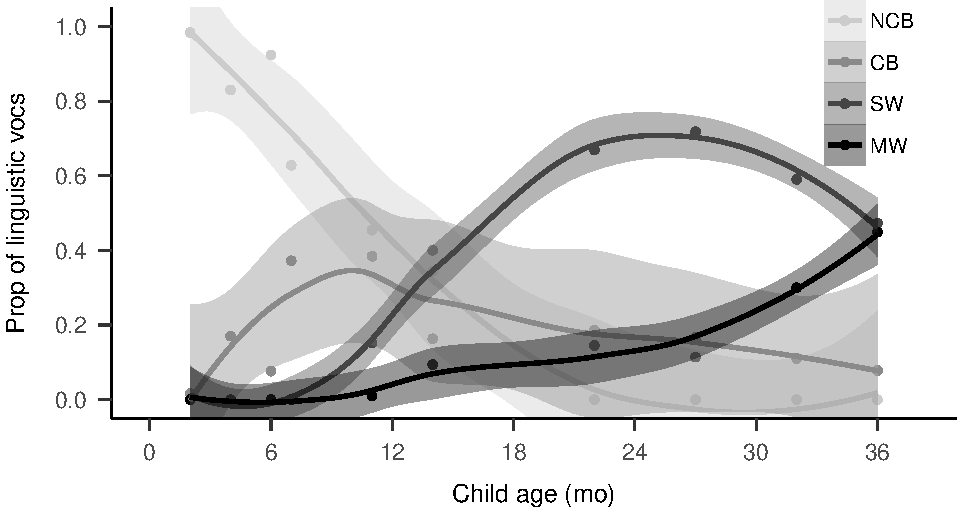
\includegraphics{Tseltal-CLE_files/figure-latex/fig6-1.pdf}
\caption{\label{fig:fig6}Proportion of vocalization types used by children
across age (NCB = Non-canonical babble, CB = Canonical babble, SW =
single word utterance, MW = multi-word utterance).}
\end{figure}

\subsubsection{Frequency of
vocalizations}\label{frequency-of-vocalizations}

We can use these same data to roughly infer how \emph{often} children
use speech-like vocalizations (i.e., \enquote{usage} instead of
\enquote{onset} measures; Warlaumont et al. (2014); retracted for
review). These 6 Tseltal children, between 2 and 14 months, demonstrated
a large increase in the proportion of speech-like vocalizations
(canonical babbling and lexical speech): from 9\% before 0;6 to 58\%
between 0;10 and 1;2. Notably, this usage rate for speech-like syllables
far exceeds the threshold associated with later language delay in
American infants (Oller et al., 1998). There is very little published
data with which we can compare these patterns, but we see that around
age 1;0, the Tseltal children's use of speech-like vocalizations (58\%)
is nearly identical to that reported by Warlaumont et al. (2014) for
American children around age 1;0 in an socioeconomically diverse sample
(approximately 60\%). Further, in a separate study, a subset of these
Tseltal vocalizations have been independently re-annotated and compared
to vocalizations from children acquiring five other non-related
languages, with very similar results: the ratio of speech-like
vocalizations to all linguistic vocalizations (canonical babbling ratio,
e.g., Lee et al., 2018) increases similarly under a variety of different
linguistic and childrearing environments between ages 0;2 and 3;0,
during which time children in all six communities begin to produce their
first words and multi-word utterances (retracted for review).

We also found that, in general, the Tseltal children did not vocalize
very often: they produced an average of 7.88 linguistic vocalizations
per minute (median = 7.55; range = 4.08--12.55) during their full one
hour of annotated audio (including the high vocal activity minutes), not
including crying and laughter. This rate is consistent with prior
estimates for the frequency of child-initiated prompts in Tseltal
interaction (Brown, 2011). Given that our age range goes all the way up
to 3;0, this rate is perhaps lower than what would be expected based on
recordings made in the lab with American infant-caregiver pairs (Oller
et al., 1995), in which a rate of 6--9 vocalizations per minute was
already evident at 16 months across a socioeconomically diverse sample.
The lower rate of vocalization in Tseltal is consistent with caregivers'
encouragement that children attend to the events going on around them,
but is also in-line with the idea that rate of vocalization is sensitive
to the language environment (Oller et al., 1995; Warlaumont et al.,
2014). However, vocalization rate estimates from daylong recordings
would be necessary to more validly make this comparison.

\hypertarget{disc}{\section{Discussion}\label{disc}}

We analyzed 10 Tseltal Mayan children's speech environments to find out
how often they had the opportunity to attend and respond to speech and
to also sketch out a basic trajectory of their early vocal development.
Based on prior work, we predicted infrequent and non-uniform use of TCDS
throughout the day, an increase in TCDS with child age, and that a large
proportion of children's TCDS would come from other children. We had
also predicted that children's vocal development would show no obvious
signs of delay compared to similar benchmarks in Western children. Only
some of these predictions were borne out in the analyses. We did find
evidence for infrequent use of TCDS and for its non-uniform use over the
day; as predicted, children were most likely to hear speech in the
mornings and afternoons---times of day when the household members are
likely to be gathered for meals and socializing. Relatedly, the sheer
number of speakers present a robust predictor of the quantity of ODS the
children heard, above and beyond the time of day. We also saw that
Tseltal children's speech showed approximately similar benchmark ages
for the onset of canonical babble, first words, and first word
combinations based on Western children's data. These findings indicate
no obvious delay in development: Tseltal children are able to extract
enough information from their linguistic environments to produce at
least some words and multi-word utterances at comparable ages to the
emergence of those behaviors in Western children.

That said, we did \emph{not} find evidence that an increasing majority
of TCDS comes from other children. Instead, we saw that the majority of
TCDS came from adults, and that the quantity of directed speech from
both adults and children was stable across the first three years of
life. The present findings therefore only partly replicate estimates of
child language input in previous work on Yucatec Mayan and Tseltal Mayan
communities (Yucatec: Shneidman \& Goldin-Meadow 2012; Tseltal: Brown,
1998, 2011, 2014), and bring new questions to light regarding the
distribution of child-directed speech over activities and interactant
types in Mayan children's speech environments.

\subsection{Learning Tseltal with little child-directed
speech}\label{learning-tseltal-with-little-child-directed-speech}

A main goal of our analysis was to find out how much speech Tseltal
children hear: we wanted to know how often they were directly spoken to
and how often they might have been able to listen to speech directed to
others. Consistent with prior work, the children were only infrequently
directly spoken to: a day-wide average of 3.63 minutes per hour in the
random sample. This average TCDS rate for Tseltal is approximately a
third of that found for North American children (Bergelson et al.,
2019), but is comparable to that for Tsimane children (Scaff et al., in
preparation) and Yucatec Mayan children (Shneidman \& Goldin-Meadow,
2012) in a similar age range. Meanwhile, we found that the children
heard an enormous quantity of other-directed speech in their
environment, averaging 21.05 minutes per hour in the random sample,
which is more than has been previously reported for other cultural
settings (e.g., Bergelson et al., 2019; Scaff et al., in preparation).
In a nutshell, our findings from daylong recordings confirm prior claims
that Tseltal children, like other Mayan children, are infrequently
directly spoken to. Again, despite this, Tseltal children somehow
extract enough information about their language to produce at least some
canonical babbles, single words, and multi-word utterances at
approximately the same ages that Western children do. The important
question is then: how do children manage to extract the information they
need from their language environments without frequent TCDS?

\subsubsection{Other-directed speech}\label{other-directed-speech}

One proposal is that Mayan children become experts at observing and
learning from the interactions and behaviors taking place around them
(de León, 2011; Rogoff et al., 2003; Shneidman, 2010; Shneidman \&
Goldin-Meadow, 2012). In the randomly selected clips, children were
within hearing distance of other-directed speech for an average of 21.05
minutes per hour. This large quantity of ODS is likely due to the fact
that Tseltal children tend to live in households with more people than
the typical North American child does (Shneidman \& Goldin-Meadow,
2012). Two factors in our analysis impacted the quantity of ODS children
heard: the presence of more speakers was associated with more ODS, but
older children heard less ODS than younger ones. This latter
effect---that older children hear less ODS---is boosted by the
complementary finding that older children are more likely to hear TCDS
when more speakers are around, compared to younger children. Together,
these results ring true with Brown's (2011, 2014) claim that this
Tseltal community is non-child-centric; the presence of more people
primarily increases talk between those people (i.e., not to young
children). But, as children become more sophisticated language users,
they are more likely to participate in others' talk or perhaps walk away
from the other-directed talk to seek other activities. This latter
hypothesis is, in fact, similar to one proposed for North American
children based on manual annotations of daylong audio recordings
(Bergelson et al., 2019). We also saw that, during the interactional
peaks, children in larger households heard significantly less ODS. This
effect goes against expectations, but may reflect both our relatively
small sample (10 children) and the fact that household size is a less
stable proxy for overheard speech than the number of speakers, which
shows consistent strong effects on ODS in both the random and the
turn-taking samples. The sum of evidence, in our view, does not support
the idea that Tseltal children's early vocal development relies heavily
on ODS. First, it is most frequent when children are youngest and, if
anything, we see less ODS at later ages, when children are independently
mobile. Second, an increase in the number of speakers is also likely
associated with an increase in the amount of overlapping speech, which
likely presents additional processing difficulties (see Scaff et al., in
preparation). Third, just because speech is hearable does not mean the
children are attending to it; follow-up work on the role of ODS in
language development must better define what constitutes likely
\enquote{listened to} speech by the child. For now, we suggest that
attention to ODS is unlikely to be a primary mechanism driving early
Tseltal development.

\subsubsection{Increased TCDS with age}\label{increased-tcds-with-age}

Another possibility is that speakers more frequently address children
who are more communicatively competent (i.e., increased TCDS with age,
e.g., Warlaumont et al., 2014). In their longitudinal study of Yucatec
Mayan children, Shneidman and Goldin-Meadow (2012) found that TCDS
increased tremendously with age, though most of the increase came from
other children speaking to the target child. Their finding is consistent
with other reports that Mayan children are more often cared for by their
older siblings from later infancy onward (2011, 2014). In our data,
there was no evidence for an overall increase in TCDS with age, neither
from adult speakers nor from child speakers. This non-increase in TCDS
with age may be due to the fact that TCDS from other children was,
overall, simply rare in our data. TCDS from other children may have been
rare because: (a) the target children were relatively young and so spent
much of their time with their mothers, (b) these particular children did
not have many older siblings, and (c) in the daylong recording context
more adults were present to talk to each other than would be typical in
a short-format recording (as used in Shneidman \& Goldin-Meadow, 2012).
That aside, we conclude for now that an increase in TCDS with age is
also unlikely to be a primary mechanism driving early Tseltal
development.

\subsubsection{Learning during interactional
bursts}\label{learning-during-interactional-bursts}

A third possibility is that children learn effectively from short,
routine language encounters. Bursty input appears to be the norm across
a number of linguistic and interactive scales (e.g., Abney et al., 2017;
Blasi et al., in preparation), and experiment-based work suggests that
children can benefit from massed presentation of new information (Schwab
\& Lew-Williams, 2016). We propose two mechanisms through which Tseltal
children might capitalize on the distribution of speech input in their
environment: (a) they experience most language input during routine
activities, giving them a more constrained, predictable entry into early
interaction (b) they consolidate their language experiences during the
downtime between interactive peaks. Neither of these mechanisms are
proposed to be particular to Tseltal children, but might be employed to
help explain their language development without frequent CDS.

Tseltal children's linguistic input is not uniformly distributed over
the day: children were most likely to encounter directed, contingent
speech in the mornings. Older children, who are less often carried and
were therefore probably more free to seek out interactions, showed these
time of day effects more strongly, eliciting TCDS both in the mornings
(when the entire household was likely present) \emph{and} around midday
(when many people had likely dispersed for work), and hearing less ODS
overall and less ODS in the presence of other speakers compared to
younger children (see also Bergelson et al., 2019). Prior work with
North American children's daylong recordings has also shown a decrease
in environmental speech just after midday (Greenwood et al., 2011;
Soderstrom \& Wittebolle, 2013). Similar time of day effects across
multiple cultural contexts could arise from coincidental similarities in
the types of activities that occur in the mornings and afternoons, for
example, morning meal gatherings or short bouts of infant sleep
(Soderstrom \& Wittebolle, 2013). That said, in the North American data
(Soderstrom \& Wittebolle, 2013), the highest density speech input came
during storytime and organized playtime (e.g., sing-alongs, painting),
while mealtime was associated with less speech. We expect that follow-up
research tracking TCDS during activities in Tseltal will lead to very
different conclusions: storytime and organized playtime are vanishingly
rare in this non-child-centric community, and mealtime may represent a
time of routine and rich linguistic experience. In both cases, however,
the underlying association with activity (not hour) implies a role for
action routines that help children optimally extract information about
what words, agents, objects, and actions they will encounter and what
they are expected to do in response (see, e.g., Bruner, 1983;
Tamis-LeMonda et al., 2018). Our study is the first to show these time
of day effects in a subsistence farming community, and to show that time
of day effects differ depending on child age and that time of day
differentially affects CDS and ODS. That said, without actual
information about the ongoing activities in each household (as in
Soderstrom \& Wittebolle, 2013) we cannot accurately assess the
potential role of routine in Tseltal language development.

A more speculative possibility is that Tseltal children learn language
on a natural input-consolidation cycle: the rarity of interactional
peaks throughout the day may be complemented by an opportunity to
consolidate new information. Sleep has been shown to benefit language
learning tasks in both adults (Frost \& Monaghan, 2017; Mirković \&
Gaskell, 2016) and children (Gómez, Bootzin, \& Nadel, 2006; Horváth,
Liu, \& Plunkett, 2016; Hupbach, Gómez, Bootzin, \& Nadel, 2009),
including word learning, phonotactic constraints, and syntactic
structure. Our impression, both from the recordings and informal
observations made during visits to the community, is that young Tseltal
children frequently sleep for short periods throughout the day,
particularly at younger ages when they spend much of their day wrapped
within the shawl on their mother's back. Mayan children tend to pick
their own breastfeeding and resting times; there are no formalized
\enquote{sleep} times, even at night (Morelli, Rogoff, Oppenheim, \&
Goldsmith, 1992), and Mayan mothers take special care to keep infants in
a calm and soothing environment in the first few months of life (e.g.,
de León, 2011; Pye, 1986). There is little quantitative data on Mayan
children's daytime and nighttime sleeping patterns, but one study
estimates that Yucatec Mayan children between 0;0 and 2;0 sleep or rest
approximately 15\% of the time between morning and evening (Gaskins,
2000), doing so at times that suited the child (Morelli et al., 1992).
If Tseltal children's interactional peaks are bookended by short
sleeping periods, it could contribute to efficient consolidation of new
information encountered. How often Tseltal children sleep, how deeply,
and how their sleeping patterns may relate to their linguistic
development is an important topic for future research.

\subsection{Limitations and Future Work}\label{disc-limfut}

The current findings are based on a cross-sectional analysis of 600
annotated recording minutes, divided among only ten children. The data
are limited to verbal activity; we cannot analyze gaze and gestural
behavior. We have also used very coarse indices of language development
in a small, cross-sectional sample with little existing data to which we
can make direct comparisons (but see Oller et al., 1998; Warlaumont et
al., 2014; retracted for review). More detailed measures of
phonological, lexical, and syntactic growth will be crucial for shedding
light on the relation between what Tseltal children hear and how they
develop early language skills, building on past work (Brown, 1998, 2011,
2014; Brown \& Gaskins, 2014). In short, more and more diverse data are
needed to enrich this initial description of Tseltal children's language
environments. Importantly, the current analyses are based on a corpus
that is still under active development. As new data, annotations, and
analyses are added, up-to-date summaries of TCDS, ODS, early speech, and
more will be available at:
\url{https://retracted_for_review.shinyapps.io/retracted_for_review/}.

\subsection{Conclusion}\label{disc-conclusion}

We estimate that, over the course of a waking day, Tseltal children
under age 3;0 hear an average of 3.63 minutes of directed speech per
hour. However, during their peak moments of interactivity, children hear
TCDS at an average rate of 13.28 minutes per hour, and the quantity of
speech they hear is influenced by the time of day, both on its own and
in combination with the child's age. Despite the fact that children hear
infrequent TCDS, our preliminary measures of the onset of canonical
babble, first words, and first word combinations show no delay compared
to Western norms. These findings raising a challenge for future work:
how do Tseltal children efficiently extract the information they need
from their linguistic environments? In our view, a promising avenue for
continued research is to more closely investigate how directed speech is
distributed over daily activities and to explore a possible
input-consolidation cycle for language exposure in early development. By
better understanding how children in this community learn Tseltal, we
hope to help uncover how human language learning mechanisms are adaptive
to the many thousands of ethnolinguistic environments in which children
develop.

\section{Acknowledgements}\label{acknowledgements}

Retracted for review

\newpage

\section{References}\label{refs}

\begingroup
\setlength{\parindent}{-0.5in} \setlength{\leftskip}{0.5in}

\hypertarget{refs}{}
\hypertarget{ref-abney2017time}{}
Abney, D. H., Smith, L. B., \& Yu, C. (2017). It's time: Quantifying the
relevant time scales for joint attention. In G. Gunzelmann, A. Howes, T.
Tenbrink, \& E. Davelaar (Eds.), \emph{Proceedings of the 39th Annual
Meeting of the Cognitive Science Society} (pp. 1489--1494). London, UK.

\hypertarget{ref-bergelson2018day}{}
Bergelson, E., Amatuni, A., Dailey, S., Koorathota, S., \& Tor, S.
(2018). Day by day, hour by hour: Naturalistic language input to
infants. \emph{Developmental Science}, \emph{22}(1), e12715.
doi:\href{https://doi.org/10.1111/desc.12715}{10.1111/desc.12715}

\hypertarget{ref-bergelsoncasillas2019what}{}
Bergelson, E., Casillas, M., Soderstrom, M., Seidl, A., Warlaumont, A.
S., \& Amatuni, A. (2019). What do North American babies hear? A
large-scale cross-corpus analysis. \emph{Developmental Science},
\emph{22}(1), e12724.
doi:\href{https://doi.org/10.1111/desc.12724}{10.1111/desc.12724}

\hypertarget{ref-blasiIPhuman}{}
Blasi, D., Schikowski, R., Moran, S., Pfeiler, B., \& Stoll, S. (in
preparation). Human communication is structured efficiently for first
language learners: Lexical spikes.

\hypertarget{ref-brinchmann2019direct}{}
Brinchmann, E. I., Braeken, J., \& Lyster, S.-A. H. (2019). Is there a
direct relation between the development of vocabulary and grammar?
\emph{Developmental Science}, \emph{22}(1), e12709.
doi:\href{https://doi.org/10.1111/desc.12709}{10.1111/desc.12709}

\hypertarget{ref-brooks2017modeling}{}
Brooks, M. E., Kristensen, K., van Benthem, K. J., Magnusson, A., Berg,
C. W., Nielsen, A., \ldots{} Bolker, B. M. (2017). Modeling
zero-inflated count data with glmmTMB. \emph{bioRxiv}.
doi:\href{https://doi.org/10.1101/132753}{10.1101/132753}

\hypertarget{ref-brown1998conversational}{}
Brown, P. (1998). Conversational structure and language acquisition: The
role of repetition in Tzeltal adult and child speech. \emph{Journal of
Linguistic Anthropology}, \emph{2}, 197--221.
doi:\href{https://doi.org/10.1525/jlin.1998.8.2.197}{10.1525/jlin.1998.8.2.197}

\hypertarget{ref-brown2011cultural}{}
Brown, P. (2011). The cultural organization of attention. In A. Duranti,
E. Ochs, \& and B. B. Schieffelin (Eds.), \emph{Handbook of Language
Socialization} (pp. 29--55). Malden, MA: Wiley-Blackwell.

\hypertarget{ref-brown2014interactional}{}
Brown, P. (2014). The interactional context of language learning in
Tzeltal. In I. Arnon, M. Casillas, C. Kurumada, \& B. Estigarribia
(Eds.), \emph{Language in interaction: Studies in honor of Eve V. Clark}
(pp. 51--82). Amsterdam, NL: John Benjamins.

\hypertarget{ref-brown2014language}{}
Brown, P., \& Gaskins, S. (2014). Language acquisition and language
socialization. In N. J. Enfield, P. Kockelman, \& J. Sidnell (Eds.),
\emph{Handbook of Linguistic Anthropology} (pp. 187--226). Cambridge,
UK: Cambridge University Press.
doi:\href{https://doi.org/10.1017/CBO9781139342872.010}{10.1017/CBO9781139342872.010}

\hypertarget{ref-bruner1983childs}{}
Bruner, J. (1983). \emph{Child's talk}. Oxford: Oxford University Press.
doi:\href{https://doi.org/10.1177/026565908500100113}{10.1177/026565908500100113}

\hypertarget{ref-cartmill2013quality}{}
Cartmill, E. A., Armstrong, B. F., Gleitman, L. R., Goldin-Meadow, S.,
Medina, T. N., \& Trueswell, J. C. (2013). Quality of early parent input
predicts child vocabulary 3 years later. \emph{Proceedings of the
National Academy of Sciences}, \emph{110}(28), 11278--11283.
doi:\href{https://doi.org/10.1073/pnas.1309518110}{10.1073/pnas.1309518110}

\hypertarget{ref-casillas2017ACLEWDAS}{}
Casillas, M., Bunce, J., Soderstrom, M., Rosemberg, C., Migdalek, M.,
Alam, F., \ldots{} Garrison, H. (2017). Introduction: The ACLEW DAS
template {[}training materials{]}. Retrieved from
\url{https://osf.io/aknjv/}

\hypertarget{ref-cristia2017child}{}
Cristia, A., Dupoux, E., Gurven, M., \& Stieglitz, J. (2017).
Child-directed speech is infrequent in a forager-farmer population: A
time allocation study. \emph{Child Development}, \emph{Early View},
1--15. doi:\href{https://doi.org/10.1111/cdev.12974}{10.1111/cdev.12974}

\hypertarget{ref-deleon2011language}{}
de León, L. (2011). Language socialization and multiparty participation
frameworks. In A. Duranti, E. Ochs, \& and B. B. Schieffelin (Eds.),
\emph{Handbook of Language Socialization} (pp. 81--111). Malden, MA:
Wiley-Blackwell.
doi:\href{https://doi.org/10.1002/9781444342901.ch4}{10.1002/9781444342901.ch4}

\hypertarget{ref-frankIPvariability}{}
Frank, M. C., Braginsky, M., Marchman, V. A., \& Yurovsky, D. (in
preparation). \emph{Variability and consistency in early language
learning: The Wordbank project}. Retrieved from
\url{https://langcog.github.io/wordbank-book/}

\hypertarget{ref-frost2017sleep}{}
Frost, R. L. A., \& Monaghan, P. (2017). Sleep-driven computations in
speech processing. \emph{PloS One}, \emph{12}(1), e0169538.
doi:\href{https://doi.org/10.1371/journal.pone.0169538}{10.1371/journal.pone.0169538}

\hypertarget{ref-gaskins2000childrens}{}
Gaskins, S. (2000). Children's daily activities in a Mayan village: A
culturally grounded description. \emph{Cross-Cultural Research},
\emph{34}(4), 375--389.
doi:\href{https://doi.org/10.1177/106939710003400405}{10.1177/106939710003400405}

\hypertarget{ref-gaskins2006cultural}{}
Gaskins, S. (2006). Cultural perspectives on infant--caregiver
interaction. In N. J. Enfield \& S. Levinson (Eds.), \emph{Roots of
Human Sociality: Culture, Cognition and Interaction} (pp. 279--298).
Oxford: Berg.

\hypertarget{ref-gomez2006naps}{}
Gómez, R. L., Bootzin, R. R., \& Nadel, L. (2006). Naps promote
abstraction in language-learning infants. \emph{Psychological Science},
\emph{17}(8), 670--674.
doi:\href{https://doi.org/10.1111/j.1467-9280.2006.01764.x}{10.1111/j.1467-9280.2006.01764.x}

\hypertarget{ref-greenwood2011assessing}{}
Greenwood, C. R., Thiemann-Bourque, K., Walker, D., Buzhardt, J., \&
Gilkerson, J. (2011). Assessing children's home language environments
using automatic speech recognition technology. \emph{Communication
Disorders Quarterly}, \emph{32}(2), 83--92.
doi:\href{https://doi.org/10.1177/1525740110367826}{10.1177/1525740110367826}

\hypertarget{ref-hart1995meaningful}{}
Hart, B., \& Risley, T. R. (1995). \emph{Meaningful Differences in the
Everyday Experience of Young American Children}. Paul H. Brookes
Publishing.

\hypertarget{ref-henrich2010beyond}{}
Henrich, J., Heine, S. J., \& Norenzayan, A. (2010). Beyond WEIRD:
Towards a broad-based behavioral science. \emph{Behavioral and Brain
Sciences}, \emph{33}(2--3), 111--135.
doi:\href{https://doi.org/10.1017/S0140525X10000725}{10.1017/S0140525X10000725}

\hypertarget{ref-hoff2003specificity}{}
Hoff, E. (2003). The specificity of environmental influence:
Socioeconomic status affects early vocabulary development via maternal
speech. \emph{Child Development}, \emph{74}(5), 1368--1378.
doi:\href{https://doi.org/10.3389/fpsyg.2015.01492}{10.3389/fpsyg.2015.01492}

\hypertarget{ref-horvath2016daytime}{}
Horváth, K., Liu, S., \& Plunkett, K. (2016). A daytime nap facilitates
generalization of word meanings in young toddlers. \emph{Sleep},
\emph{39}(1), 203--207.
doi:\href{https://doi.org/10.5665/sleep.5348}{10.5665/sleep.5348}

\hypertarget{ref-hupbach2009nap}{}
Hupbach, A., Gómez, R. L., Bootzin, R. R., \& Nadel, L. (2009).
Nap-dependent learning in infants. \emph{Developmental Science},
\emph{12}(6), 1007--1012.
doi:\href{https://doi.org/10.1111/j.1467-7687.2009.00837.x}{10.1111/j.1467-7687.2009.00837.x}

\hypertarget{ref-huttenlocher2010sources}{}
Huttenlocher, J., Waterfall, H., Vasilyeva, M., Vevea, J., \& Hedges, L.
V. (2010). Sources of variability in children's language growth.
\emph{Cognitive Psychology}, \emph{61}(4), 343--365.
doi:\href{https://doi.org/10.1016/j.cogpsych.2010.08.002}{10.1016/j.cogpsych.2010.08.002}

\hypertarget{ref-kuhl2004early}{}
Kuhl, P. K. (2004). Early language acquisition: Cracking the speech
code. \emph{Nature Reviews Neuroscience}, \emph{5}(11), 831.
doi:\href{https://doi.org/10.1038/nrn1533}{10.1038/nrn1533}

\hypertarget{ref-lee2018babbling}{}
Lee, C.-C., Jhang, Y., Relyea, G., Chen, L.-m., \& Oller, D. K. (2018).
Babbling development as seen in canonical babbling ratios: A
naturalistic evaluation of all-day recordings. \emph{Infant Behavior and
Development}, \emph{50}, 140--153.

\hypertarget{ref-lieven1997lexically}{}
Lieven, E. V. M., Pine, J. M., \& Baldwin, G. (1997). Lexically-based
learning and early grammatical development. \emph{Journal of Child
Language}, \emph{24}(1), 187--219.
doi:\href{https://doi.org/10.1017/S0305000996002930}{10.1017/S0305000996002930}

\hypertarget{ref-liszkowski2012prelinguistic}{}
Liszkowski, U., Brown, P., Callaghan, T., Takada, A., \& de Vos, C.
(2012). A prelinguistic gestural universal of human communication.
\emph{Cognitive Science}, \emph{36}(4), 698--713.
doi:\href{https://doi.org/10.1111/j.1551-6709.2011.01228.x}{10.1111/j.1551-6709.2011.01228.x}

\hypertarget{ref-manybabies2017}{}
ManyBabies Collaborative. (2017). Quantifying sources of variability in
infancy research using the infant-directed speech preference.
\emph{Advances in Methods and Practices in Psychological Science},
1--46.
doi:\href{https://doi.org/10.31234/osf.io/s98ab}{10.31234/osf.io/s98ab}

\hypertarget{ref-marchman2004language}{}
Marchman, V. A., Martínez-Sussmann, C., \& Dale, P. S. (2004). The
language-specific nature of grammatical development: Evidence from
bilingual language learners. \emph{Developmental Science}, \emph{7}(2),
212--224.
doi:\href{https://doi.org/10.1111/j.1467-7687.2004.00340.x}{10.1111/j.1467-7687.2004.00340.x}

\hypertarget{ref-mcgillion2017paves}{}
McGillion, M., Herbert, J. S., Pine, J., Vihman, M., DePaolis, R.,
Keren-Portnoy, T., \& Matthews, D. (2017). What paves the way to
conventional language? The predictive value of babble, pointing, and
socioeconomic status. \emph{Child Development}, \emph{88}(1), 156--166.

\hypertarget{ref-mirkovic2016does}{}
Mirković, J., \& Gaskell, M. G. (2016). Does sleep improve your grammar?
Preferential consolidation of arbitrary components of new linguistic
knowledge. \emph{PloS One}, \emph{11}(4), e0152489.
doi:\href{https://doi.org/10.1371/journal.pone.0152489}{10.1371/journal.pone.0152489}

\hypertarget{ref-morelli1992cultural}{}
Morelli, G. A., Rogoff, B., Oppenheim, D., \& Goldsmith, D. (1992).
Cultural variation in infants' sleeping arrangements: Questions of
independence. \emph{Developmental Psychology}, \emph{28}(4), 604.
doi:\href{https://doi.org/10.1037/0012-1649.28.4.604}{10.1037/0012-1649.28.4.604}

\hypertarget{ref-nielsen2017persistent}{}
Nielsen, M., Haun, D., Kärtner, J., \& Legare, C. H. (2017). The
persistent sampling bias in developmental psychology: A call to action.
\emph{Journal of Experimental Child Psychology}, \emph{162}, 31--38.
doi:\href{https://doi.org/10.1016/j.jecp.2017.04.017}{10.1016/j.jecp.2017.04.017}

\hypertarget{ref-ochs1984language}{}
Ochs, E., \& Schieffelin, B. (1984). Language acquisition and
socialization: Three developmental stories and their implications. In R.
A. Schweder \& R. A. LeVine (Eds.), \emph{Culture theory: Essays on
mind, self, and emotion} (pp. 276--322). Cambridge University Press.

\hypertarget{ref-oller1995extreme}{}
Oller, D. K., Eilers, R. E., Basinger, D., Steffens, M. L., \& Urbano,
R. (1995). Extreme poverty and the development of precursors to the
speech capacity. \emph{First Language}, \emph{15}(44), 167--187.

\hypertarget{ref-oller1998late}{}
Oller, D. K., Eilers, R. E., Neal, A. R., \& Cobo-Lewis, A. B. (1998).
Late onset canonical babbling: A possible early marker of abnormal
development. \emph{American Journal on Mental Retardation},
\emph{103}(3), 249--263.

\hypertarget{ref-pine1993reanalysing}{}
Pine, J. M., \& Lieven, E. V. M. (1993). Reanalysing rote-learned
phrases: Individual differences in the transition to multi-word speech.
\emph{Journal of Child Language}, \emph{20}(3), 551--571.
doi:\href{https://doi.org/10.1017/S0305000900008473}{10.1017/S0305000900008473}

\hypertarget{ref-pye1986quiche}{}
Pye, C. (1986). Quiché Mayan speech to children. \emph{Journal of Child
Language}, \emph{13}(1), 85--100.
doi:\href{https://doi.org/10.1017/S0305000900000313}{10.1017/S0305000900000313}

\hypertarget{ref-pye2017comparative}{}
Pye, C. (2017). \emph{The Comparative Method of Language Acquisition
Research}. University of Chicago Press.

\hypertarget{ref-R-base}{}
R Core Team. (2018). \emph{R: A language and environment for statistical
computing}. Vienna, Austria: R Foundation for Statistical Computing.
Retrieved from \url{https://www.R-project.org/}

\hypertarget{ref-rogoff2003firsthand}{}
Rogoff, B., Paradise, R., Arauz, R. M., Correa-Chávez, M., \& Angelillo,
C. (2003). Firsthand learning through intent participation. \emph{Annual
Review of Psychology}, \emph{54}(1), 175--203.
doi:\href{https://doi.org/10.1146/annurev.psych.54.101601.145118}{10.1146/annurev.psych.54.101601.145118}

\hypertarget{ref-rowe2008child}{}
Rowe, M. L. (2008). Child-directed speech: Relation to socioeconomic
status, knowledge of child development and child vocabulary skill.
\emph{Journal of Child Language}, \emph{35}(1), 185--205.
doi:\href{https://doi.org/10.1017/S0305000907008343}{10.1017/S0305000907008343}

\hypertarget{ref-scaffIPlanguage}{}
Scaff, C., Stieglitz, J., Casillas, M., \& Cristia, A. (in preparation).
Language input in a hunter-forager population: Estimations from daylong
recordings.

\hypertarget{ref-schwab2016repetition}{}
Schwab, J. F., \& Lew-Williams, C. (2016). Repetition across successive
sentences facilitates young children's word learning.
\emph{Developmental Psychology}, \emph{52}(6), 879--886.
doi:\href{https://doi.org/10.1037/dev0000125}{10.1037/dev0000125}

\hypertarget{ref-shneidman2010language}{}
Shneidman, L. A. (2010). \emph{Language Input and Acquisition in a Mayan
Village} (PhD thesis). The University of Chicago.

\hypertarget{ref-shneidman2012language}{}
Shneidman, L. A., \& Goldin-Meadow, S. (2012). Language input and
acquisition in a Mayan village: How important is directed speech?
\emph{Developmental Science}, \emph{15}(5), 659--673.
doi:\href{https://doi.org/10.1111/j.1467-7687.2012.01168.x}{10.1111/j.1467-7687.2012.01168.x}

\hypertarget{ref-slobin1970universals}{}
Slobin, D. I. (1970). Universals of grammatical development in children.
In G. B. Flores d'Arcais \& W. J. M. Levelt (Eds.), \emph{Advances in
Psycholinguistics} (pp. 174--186). Amsterdam, NL: North Holland
Publishing.

\hypertarget{ref-smithson2013generalized}{}
Smithson, M., \& Merkle, E. (2013). \emph{Generalized linear models for
categorical and continuous limited dependent variables}. New York:
Chapman; Hall/CRC.
doi:\href{https://doi.org/10.1201/b15694}{10.1201/b15694}

\hypertarget{ref-soderstrom2007beyond}{}
Soderstrom, M. (2007). Beyond babytalk: Re-evaluating the nature and
content of speech input to preverbal infants. \emph{Developmental
Review}, \emph{27}(4), 501--532.
doi:\href{https://doi.org/10.1016/j.dr.2007.06.002}{10.1016/j.dr.2007.06.002}

\hypertarget{ref-soderstrom2013when}{}
Soderstrom, M., \& Wittebolle, K. (2013). When do caregivers talk? The
influences of activity and time of day on caregiver speech and child
vocalizations in two childcare environments. \emph{PloS One}, \emph{8},
e80646.
doi:\href{https://doi.org/10.1371/journal.pone.0080646}{10.1371/journal.pone.0080646}

\hypertarget{ref-tamislemonda2018routine}{}
Tamis-LeMonda, C. S., Custode, S., Kuchirko, Y., Escobar, K., \& Lo, T.
(2018). Routine language: Speech directed to infants during home
activities. \emph{Child Development}, \emph{Early View}, 1--18.

\hypertarget{ref-tomasello1999early}{}
Tomasello, M., \& Brooks, P. J. (1999). Early syntactic development: A
Construction Grammar approach. In M. Barrett (Ed.), \emph{The
Development of Language} (pp. 161--190). New York: Psychology Press.

\hypertarget{ref-vogt2015communicative}{}
Vogt, P., Mastin, J. D., \& Schots, D. M. A. (2015). Communicative
intentions of child-directed speech in three different learning
environments: Observations from the Netherlands, and rural and urban
Mozambique. \emph{First Language}, \emph{35}(4--5), 341--358.
doi:\href{https://doi.org/10.1177/0142723715596647}{10.1177/0142723715596647}

\hypertarget{ref-warlaumont2014social}{}
Warlaumont, A. S., Richards, J. A., Gilkerson, J., \& Oller, D. K.
(2014). A social feedback loop for speech development and its reduction
in Autism. \emph{Psychological Science}, \emph{25}(7), 1314--1324.
doi:\href{https://doi.org/10.1177/0956797614531023}{10.1177/0956797614531023}

\hypertarget{ref-weisleder2013talking}{}
Weisleder, A., \& Fernald, A. (2013). Talking to children matters: Early
language experience strengthens processing and builds vocabulary.
\emph{Psychological Science}, \emph{24}(11), 2143--2152.
doi:\href{https://doi.org/10.1177/0956797613488145}{10.1177/0956797613488145}

\hypertarget{ref-R-ggplot2}{}
Wickham, H. (2009). \emph{Ggplot2: Elegant graphics for data analysis}.
Springer-Verlag New York. Retrieved from \url{http://ggplot2.org}

\hypertarget{ref-ELAN}{}
Wittenburg, P., Brugman, H., Russel, A., Klassmann, A., \& Sloetjes, H.
(2006). ELAN: A professional framework for multimodality research. In
\emph{Proceedings of the Fifth International Conference on Language
Resources and Evaluation} (pp. 1556--1559).

\hypertarget{ref-yurovsky2018communicative}{}
Yurovsky, D. (2018). A communicative approach to early word learning.
\emph{New Ideas in Psychology}, \emph{50}, 73--79.
doi:\href{https://doi.org/10.1016/j.newideapsych.2017.09.001}{10.1016/j.newideapsych.2017.09.001}

\endgroup






\end{document}
